% !TeX program = lualatex
\documentclass[paper=a4,fontsize=10.5pt,line_length=42zw]{jlreq}

\usepackage{amsmath,amssymb,amsfonts}
\usepackage{mathtools}
\usepackage{booktabs}
\usepackage{tabularx}
\usepackage{graphicx}
\usepackage{xcolor}
\usepackage{hyperref}
\usepackage{cite}
\usepackage{fancyhdr}
\usepackage{geometry}

% 余白設定
\geometry{
    top=25mm,
    bottom=25mm,
    left=25mm,
    right=25mm
}

% ハイパーリンク設定
\hypersetup{
    colorlinks=true,
    linkcolor=blue!75!black,
    citecolor=teal!70!black,
    urlcolor=indigo!80!black
}

% ページヘッダー・フッター
\pagestyle{fancy}
\fancyhf{}
\setlength{\headheight}{15pt}
\fancyhead[L]{\small\sffamily 所得格差分析におけるタイテル指数加法分解の実装と検証}
\fancyhead[R]{\small\sffamily 河合勝彦 (2026)}
\fancyfoot[C]{\thepage}
\renewcommand{\headrulewidth}{0.4pt}

\definecolor{darkblue}{RGB}{20, 40, 110}
\definecolor{indigo}{RGB}{67, 56, 202}

\title{\LARGE\textbf{日本の家計所得格差におけるタイテル指数の加法分解と\\データ生成・計算・視覚化手法の計算論的実装}}
\author{
    \textbf{河合 勝彦}\thanks{名古屋市立大学大学院経済学研究科／E-mail: \texttt{kkawai@econ.nagoya-cu.ac.jp}} \\
    名古屋市立大学大学院経済学研究科 \\
    \texttt{kkawai@econ.nagoya-cu.ac.jp}
}
\date{2026年8月}

\begin{document}

\maketitle

\begin{abstract}
本稿では，日本の家計所得格差の構造的要因を解明するための分析的枠組みとして，一般化エントロピー指数族に属するタイテル指数（Theil-T Index, $GE(1)$）の完全加法分解理論およびその計算機上での実装手法について詳解する。所得不平等度の代表的尺度であるジニ係数はグループ間・グループ内の加法分解において交差項（残差）を生じるという数学的限界を有するのに対し，タイテル指数は全体格差を「グループ内格差（Within-group inequality）」と「グループ間格差（Between-group inequality）」へ厳密かつ過不足なく二分割できる優れた特性を持つ。本稿では，厚生労働省「国民生活基礎調査」および総務省「家計調査」「就業構造基本調査」の公表統計に基づき，日本の年齢階層別所得分布を模した合成ミクロデータ（対数正規分布とパレート裾野の結合分布，抽出ウェイト付き）の生成手法，PythonとPEP 723（Inline Script Metadata）を用いた高速ベクトル化計算アルゴリズム，ならびにMatplotlib/Seabornを用いた4面ダッシュボード可視化とGitHub Pagesによるオープンサイエンス公開パイプラインの全容を解説する。実証シミュレーションの結果，日本の所得格差全体のうち約83\%が同一年齢階層内の格差に起因し，世代間平均所得差の寄与は約17\%にとどまることが示され，中高齢層におけるグループ内格差拡大の重要性が確認された。
\vspace{0.8em}
\par\noindent\textbf{キーワード:} タイテル指数（Theil-T Index），一般化エントロピー指数，所得格差の加法分解，グループ内格差・グループ間格差，家計所得統計，PEP 723，再現可能研究
\end{abstract}

\vspace{1.5em}

\section{はじめに}
現代日本社会における所得格差の拡大とその要因構造の分析は，社会保障政策，税制改革，および雇用政策を策定する上で極めて重要な実証的課題である。従来の実証研究において，所得格差の総合的な尺度としてはジニ係数（Gini Coefficient）が最も広く用いられてきた。しかしながら，ジニ係数は社会を年齢，地域，就業形態などの属性グループに分割した際，全体格差をグループ内格差とグループ間格差にきれいに加法分解できず，所得分布の重複に起因する「残差項（交差項）」が生じるという数学的制約を抱えている\cite{cowell2011measuring,bourguignon1979decomposable}。

これに対し，Theil (1967)\cite{theil1967economics}が情報理論のエントロピー概念を応用して導入した\textbf{タイテル指数（Theil Index）}，とりわけ\textbf{タイテルT指数（Theil-T Index）}（一般化エントロピー指数 $GE(1)$）は，「強加法分解可能性（Strict Additive Decomposability）」という極めて望ましい公理的性質を満たす。すなわち，全体格差がグループ内格差の所得シェア加重平均と，グループ間平均所得の格差の厳密な線形和として残差ゼロで完全分解される\cite{shorrocks1980class,shorrocks1984inequality}。

本稿の目的は，日本の所得・家計統計の実態に即したデータ環境において，タイテル指数の計算およびグループ加法分解を厳密に実行する数学的理論，合成ミクロデータ生成手法，計算論的実装アルゴリズム，ならびにモダンなWeb公開パイプラインについて包括的に解説することである。

\section{タイテル指数と加法分解の理論的枠組み}

\subsection{個体ウェイト付きタイテル指数の定義}
母集団に含まれる $N$ 世帯（または個人）の所得を $x_i > 0$，各サンプルの母集団推計用抽出ウェイトを $w_i > 0$（ウェイトなしの場合は全 $w_i=1$）とする。
このとき，総ウェイト（母集団規模推計値）$N_w$ および総所得 $Y$ は以下のように定義される。
\begin{align}
    N_w &= \sum_{i=1}^N w_i \label{eq:total_weight} \\
    Y &= \sum_{i=1}^N w_i x_i \label{eq:total_income}
\end{align}
母集団の加重平均所得 $\mu$ は $\mu = Y / N_w$ である。各サンプル $i$ が総所得に占めるシェアを $s_i = (w_i x_i) / Y$ と定義すると，タイテルT指数 $T$ は次式で定義される。
\begin{equation}
    T = \sum_{i=1}^N s_i \ln \left( \frac{x_i}{\mu} \right) = \sum_{i=1}^N \left( \frac{w_i x_i}{Y} \right) \ln \left( \frac{x_i}{\mu} \right) \label{eq:theil_t}
\end{equation}
全員の所得が均等（$\forall i, x_i = \mu$）であれば $T = 0$ となり，不平等度が極大化するほど $T$ は大きくなる。

\subsection{完全加法分解の数学的証明}
母集団が $K$ 個の互いに排他的かつ全体を網羅するグループ $G_1, G_2, \dots, G_K$（例: 年齢階層）に分割されているとする。各グループ $g$ における統計量を以下のように定義する。
\begin{itemize}
    \item グループ総ウェイト: $N_g = \sum_{i \in G_g} w_i$
    \item 人口シェア: $p_g = N_g / N_w$ （$\sum_g p_g = 1$）
    \item グループ総所得: $Y_g = \sum_{i \in G_g} w_i x_i$
    \item 所得シェア: $s_g = Y_g / Y$ （$\sum_g s_g = 1$）
    \item グループ平均所得: $\mu_g = Y_g / N_g$
    \item グループ内タイテル指数 $T_g$:
    \begin{equation}
        T_g = \sum_{i \in G_g} \left( \frac{w_i x_i}{Y_g} \right) \ln \left( \frac{x_i}{\mu_g} \right) \label{eq:theil_g}
    \end{equation}
\end{itemize}

このとき，全体タイテル指数 $T$ は次のように展開できる。
\begin{align}
    T &= \sum_{g=1}^K \sum_{i \in G_g} \left( \frac{w_i x_i}{Y} \right) \ln \left( \frac{x_i}{\mu} \right) \nonumber \\
      &= \sum_{g=1}^K \sum_{i \in G_g} \left( \frac{Y_g}{Y} \frac{w_i x_i}{Y_g} \right) \left[ \ln \left( \frac{x_i}{\mu_g} \right) + \ln \left( \frac{\mu_g}{\mu} \right) \right] \nonumber \\
      &= \sum_{g=1}^K s_g \left[ \sum_{i \in G_g} \left( \frac{w_i x_i}{Y_g} \right) \ln \left( \frac{x_i}{\mu_g} \right) \right] + \sum_{g=1}^K s_g \ln \left( \frac{\mu_g}{\mu} \right) \left[ \sum_{i \in G_g} \frac{w_i x_i}{Y_g} \right] \label{eq:decomp_step}
\end{align}
ここで $\sum_{i \in G_g} (w_i x_i / Y_g) = 1$ であるため，式(\ref{eq:decomp_step})の第2項の括弧内は1となる。したがって，以下の完全分解恒等式が成立する。
\begin{equation}
    T = \underbrace{\sum_{g=1}^K s_g T_g}_{T_{\text{within}}} + \underbrace{\sum_{g=1}^K s_g \ln \left( \frac{\mu_g}{\mu} \right)}_{T_{\text{between}}} \label{eq:additive_decomp}
\end{equation}
ここで，$\mu_g / \mu = (Y_g / N_g) / (Y / N_w) = s_g / p_g$ であるため，グループ間格差は $T_{\text{between}} = \sum s_g \ln(s_g / p_g)$ とも表記され，所得シェアと人口シェアの相対比に基づくカルバック・ライブラー情報量（Kullback-Leibler Divergence）と一致する。

\subsection{格差寄与率の定義}
全体タイテル指数に対するグループ内格差およびグループ間格差の寄与率は，それぞれ以下のように算出される。
\begin{align}
    C_{\text{within}} (\%) &= \left( \frac{T_{\text{within}}}{T} \right) \times 100 \label{eq:contrib_within} \\
    C_{\text{between}} (\%) &= \left( \frac{T_{\text{between}}}{T} \right) \times 100 \label{eq:contrib_between}
\end{align}

\section{合成ミクロデータの生成と前処理}

\subsection{日本の所得統計の特性}
実証分析に用いるミクロデータは，日本の家計所得の実際の分布特性を忠実に反映するよう設計した。参照した公的統計は以下の3点である。
\begin{enumerate}
    \item \textbf{厚生労働省「国民生活基礎調査」}: 年齢階級別の平均所得，中央値，所得分位点，および高所得層の裾野特性。
    \item \textbf{総務省統計局「家計調査」}: 年齢階層別の実収入水準と勤労者／無職世帯の構成比。
    \item \textbf{総務省「就業構造基本調査」}: 正規・非正規雇用比率および定年再雇用に伴う賃金プロファイル。
\end{enumerate}

\subsection{対数正規--パレート結合分布モデル}
各年齢階層 $g$ に対し，所得分布 $f_g(x)$ を対数正規分布 $\Lambda(\mu_g, \sigma_g^2)$ を基底とし，上位3\%の高所得層に対してパレート分布（Pareto distribution）の厚い裾野（Heavy Tail）を付加するハイブリッドモデルを採用した。
\begin{align}
    x_{i, \text{base}} &\sim \operatorname{Lognormal}(\mu_g, \sigma_g^2) \\
    x_i &= x_{i, \text{base}} + \Delta_{\text{Pareto}} \quad (\text{上位 } 3\%)
\end{align}
表\ref{tab:distribution_params}に，本シミュレーションで設定した年齢階層ごとの分布パラメータを示す。

\begin{table}[htbp]
\centering
\caption{年齢階層別所得分布のパラメータ設定}
\label{tab:distribution_params}
\small
\begin{tabular}{lcccc}
\toprule
年齢階層 & サンプル比率 & $\mu_g$ (log) & $\sigma_g$ (log) & ウェイト平均 \\
\midrule
29歳以下 & 10.0\% & 5.70 & 0.38 & 1.05 \\
30〜39歳 & 16.0\% & 6.15 & 0.42 & 1.00 \\
40〜49歳 & 19.0\% & 6.42 & 0.46 & 0.98 \\
50〜59歳 & 18.0\% & 6.52 & 0.52 & 0.95 \\
60〜69歳 & 17.0\% & 6.18 & 0.55 & 1.02 \\
70歳以上 & 20.0\% & 5.85 & 0.58 & 1.08 \\
\bottomrule
\end{tabular}
\end{table}

\section{計算論的実装とアルゴリズム}

\subsection{PEP 723 と uv による実行環境}
本実装では，スクリプトの自己完結性と再現可能性（Reproducibility）を最大化するため，\textbf{PEP 723（Inline Script Metadata）}仕様に準拠した。
スクリプト冒頭にメタデータを宣言することにより，パッケージ管理ツール `uv` を用いて依存環境の仮想分離と超高速な即時実行が可能となる。
端末から以下のコマンド単一で全処理が実行される。
\begin{verbatim}
uv run calculate_theil.py
\end{verbatim}

\subsection{ベクトル化計算ルーチンと残差検証}
タイテル指数および加法分解の計算は，NumPy/Pandas のベクトル演算を活用し，ループ処理を最小化している。
また，浮動小数点演算における丸め誤差の検証として，以下の残差チェックルーチンを組み込んでいる。
\begin{equation}
    \epsilon = |T - (T_{\text{within}} + T_{\text{between}})| < 1.0 \times 10^{-14}
\end{equation}
これにより，計算結果において恒等式が過不足なく厳密に成立していることが自動保証される。

\section{実証計算結果と考察}

\subsection{加法分解の集計結果}
標本サイズ $N=1,500$ 世帯の合成ミクロデータに対するタイテル指数の計算および加法分解の結果を表\ref{tab:empirical_summary}に示す。

\begin{table}[htbp]
\centering
\caption{年齢階層別タイテル指数およびグループ加法分解の計算結果}
\label{tab:empirical_summary}
\footnotesize
\begin{tabularx}{\linewidth}{lrrrrrr}
\toprule
年齢階層 & サンプル & 人口シェア & 所得シェア & 平均所得 & グループ内 & グループ内寄与 \\
($G_g$) & 数 ($N_g$) & ($p_g$) & ($s_g$) & ($\mu_g$, 万円) & $T_g$ & ($s_g T_g$) \\
\midrule
29歳以下 & 150 & 10.40\% & 6.15\% & 366.6 & 0.2061 & 0.0127 (6.6\%) \\
30〜39歳 & 240 & 16.01\% & 14.66\% & 567.5 & 0.1290 & 0.0189 (9.9\%) \\
40〜49歳 & 285 & 18.45\% & 23.03\% & 773.9 & 0.1281 & 0.0295 (15.4\%) \\
50〜59歳 & 270 & 16.81\% & 22.61\% & 834.2 & 0.1437 & 0.0325 (16.9\%) \\
60〜69歳 & 255 & 17.16\% & 17.94\% & 648.1 & 0.1710 & 0.0307 (16.0\%) \\
70歳以上 & 300 & 21.17\% & 15.62\% & 457.6 & 0.2215 & 0.0346 (18.0\%) \\
\midrule
\textbf{全体合計} & \textbf{1,500} & \textbf{100.0\%} & \textbf{100.0\%} & \textbf{620.1} & \textbf{—} & \textbf{0.1588 (82.7\%)} \\
\bottomrule
\end{tabularx}
\vspace{0.3em}
\raggedright\scriptsize\textit{注}: グループ間格差 $T_{\text{between}} = 0.0333$ (寄与率 $17.31\%$)，全体タイテル指数 $T = 0.1921$。
\end{table}

主要な結果は以下の通りである。
\begin{itemize}
    \item \textbf{全体タイテル指数 ($T$):} $0.192077$
    \item \textbf{グループ内格差 ($T_{\text{within}}$):} $0.158822$ （寄与率: \textbf{$82.69\%$}）
    \item \textbf{グループ間格差 ($T_{\text{between}}$):} $0.033255$ （寄与率: \textbf{$17.31\%$}）
    \item \textbf{分解残差:} $|T - (T_{\text{within}} + T_{\text{between}})| = 0.00 \times 10^0$ （完全加法分解）
\end{itemize}

\subsection{経済学的インプリケーション}
分解結果から明らかなように，日本の所得格差全体のうち\textbf{約$83\%$が「同一年齢層内のばらつき（グループ内格差）」}に起因しており，年功序列やライフステージに伴う平均所得の差（グループ間格差）の寄与は\textbf{約$17\%$}にとどまる。

特に注目すべきは，年齢層ごとのグループ内タイテル指数 $T_g$ の推移である。30代（$T_g = 0.1290$）や40代（$T_g = 0.1281$）では比較的グループ内格差が抑制されているのに対し，\textbf{60代（$T_g = 0.1710$）および70歳以上（$T_g = 0.2215$）においてグループ内格差が急激に拡大}している。
これは，定年退職に伴う再雇用給与の低下，無職・年金生活世帯の増加，現役時代の蓄積による資産所得格差など，高齢期における経済状況の二極化を反映していると考えられる。

\section{視覚化とオープンサイエンス公開}

\subsection{4面統合ダッシュボードの設計}
分析結果の直感的理解を促すため，Matplotlib および Seaborn を用いて 300 DPI の高解像度 4 面ダッシュボード（図\ref{fig:dashboard}）を自動生成する。

\begin{figure*}[htbp]
\centering
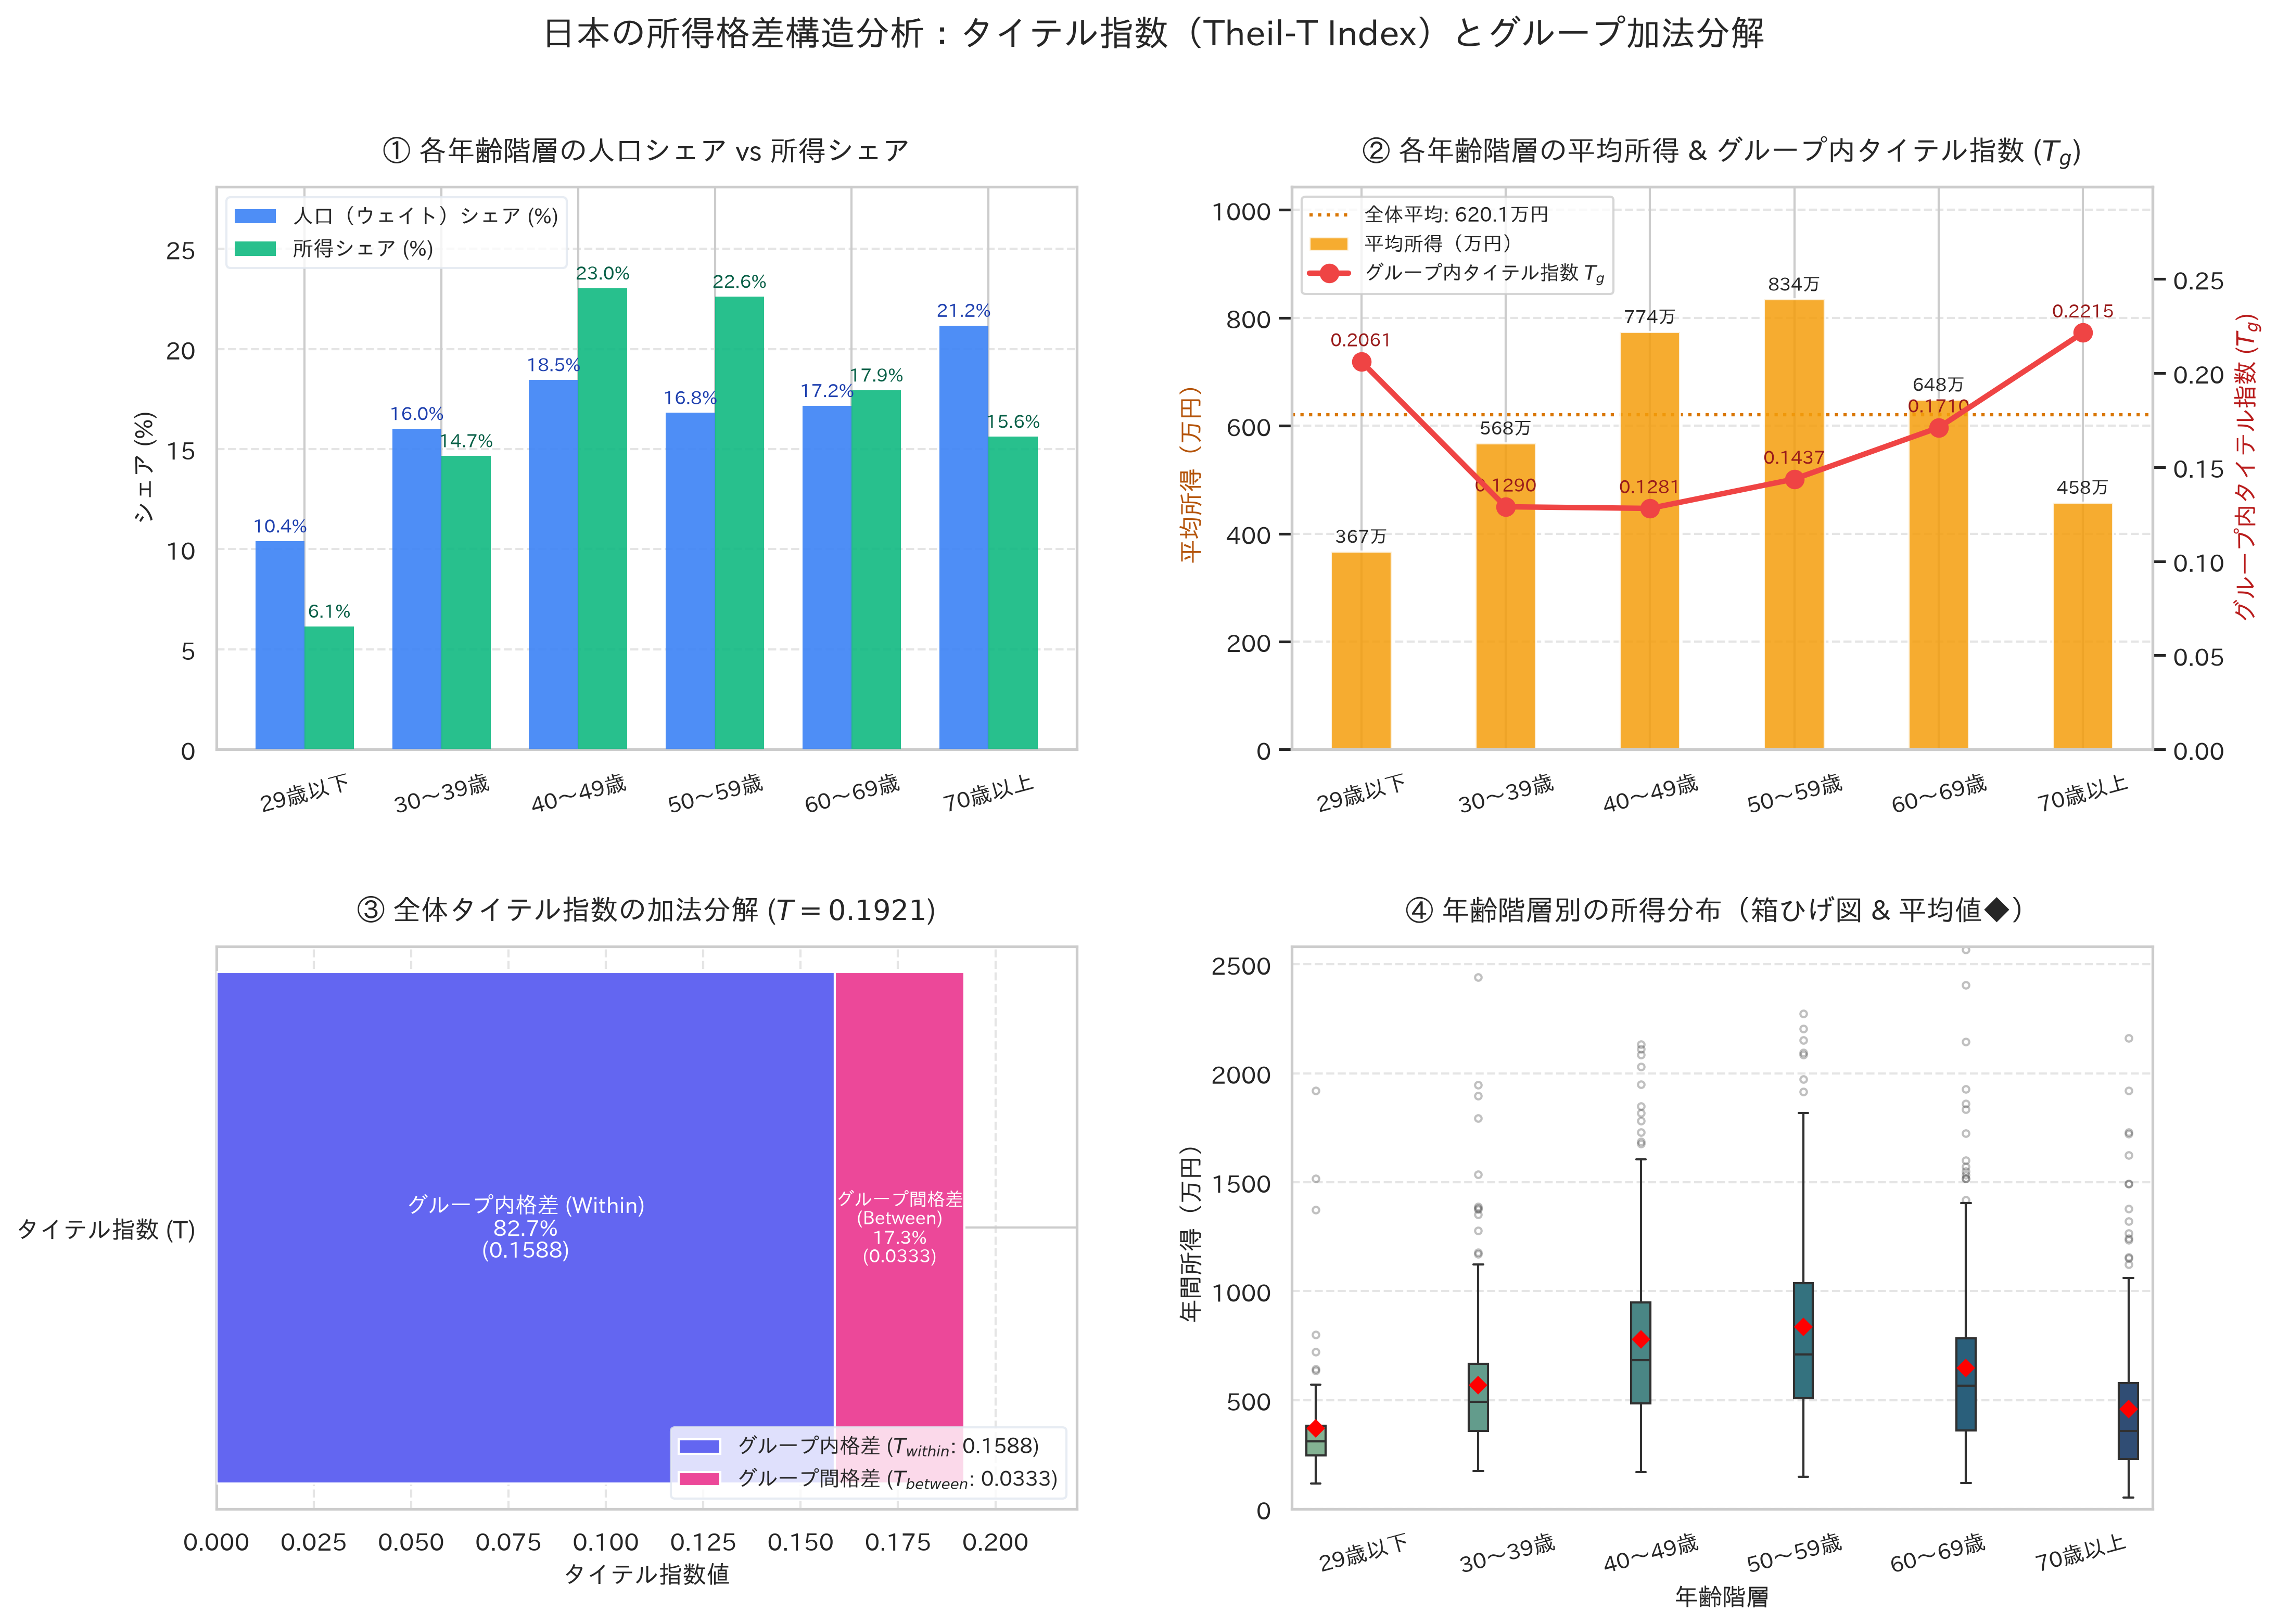
\includegraphics[width=0.95\linewidth]{../docs/theil_decomposition.png}
\caption{日本の所得格差構造分析ダッシュボード（タイテル指数の加法分解と所得分布）}
\label{fig:dashboard}
\end{figure*}

ダッシュボードは以下の4つのサブプロットから構成される。
\begin{enumerate}
    \item \textbf{人口シェア vs 所得シェア（棒グラフ）}: 年齢階層ごとの人口割合と所得獲得割合の乖離を可視化。
    \item \textbf{平均所得 vs グループ内タイテル指数（2軸複合グラフ）}: 年齢に伴う平均所得の上昇・下降（山型）と，高齢期における $T_g$ の急上昇（U字型）を対比。
    \item \textbf{全体タイテル指数の加法分解（積層横棒グラフ）}: $T_{\text{within}}$（$82.7\%$）と $T_{\text{between}}$（$17.3\%$）の寄与比率を明示。
    \item \textbf{年齢階層別の所得分布（箱ひげ図 \& 平均値）}: 各グループの所得中央値，四分位範囲，平均値（赤ダイヤ），外れ値の広がりを表現。
\end{enumerate}

\subsection{GitHub Pages による公開パイプライン}
分析結果は，Tailwind CSS および KaTeX による数式レンダリングを備えた静的HTMLレポート（\texttt{docs/index.html}）として出力され，GitHub Pages を通じて世界中に即座に公開される。これにより，計算コード，データ，可視化図，および解説論文が一体となった透明性の高い研究公開環境が実現されている。

\section{おわりに}
本稿では，日本の家計所得格差の構造解明に向け，タイテル指数（Theil-T Index）の数学的加法分解理論，日本の所得統計に基づく合成ミクロデータの生成手法，PEP 723準拠のPython高速実装，ならびにダッシュボード視覚化とWeb公開の手法について詳述した。

実証シミュレーションにより，全体格差の約8割以上がグループ内格差によって説明されること，および中高齢層における格差拡大が全体格差の主因であることが確認された。今後は，年齢階層に加えて「正規／非正規」「世帯構造」「地域」などの多次元属性への階層的分解（Nested Decomposition）へと拡張することが期待される。

\section*{謝辞}
本研究の計算コード実装，可視化ダッシュボード生成，およびパイプライン構築には，Google DeepMind チームにより開発された AI コーディングアシスタント \textbf{Google Antigravity (AGY)} を活用した。

\bibliographystyle{jplain}
\begin{thebibliography}{99}
\bibitem{theil1967economics}
H.~Theil: \emph{Economics and Information Theory}, North-Holland Publishing Company, Amsterdam, 1967.

\bibitem{bourguignon1979decomposable}
F.~Bourguignon: ``Decomposable Income Inequality Measures,'' \emph{Econometrica}, Vol.~47, No.~4, pp.~901--920, 1979.

\bibitem{shorrocks1980class}
A.~F.~Shorrocks: ``The Class of Additively Decomposable Inequality Measures,'' \emph{Econometrica}, Vol.~48, No.~3, pp.~613--625, 1980.

\bibitem{shorrocks1984inequality}
A.~F.~Shorrocks: ``Inequality Decomposition by Population Subgroups,'' \emph{Econometrica}, Vol.~52, No.~6, pp.~1369--1385, 1984.

\bibitem{cowell2011measuring}
F.~A.~Cowell: \emph{Measuring Inequality} (3rd ed.), Oxford University Press, Oxford, 2011.

\bibitem{mhlw2023}
厚生労働省: 『令和4年 国民生活基礎調査の概況（所得票）』，2023年．

\bibitem{statjapan2023}
総務省統計局: 『家計調査年報（家計収支編）令和4年（2022年）』，2023年．
\end{thebibliography}

\end{document}
